\section{Защита данных в распределенных системах}
\subsection{Распределенные вычислительные среды}
Распределённая обработка данных - методика выполнения прикладных программ группой систем.
При этом пользователь получает возможность работать с сетевыми службами и прикладными процессами,
расположенными в нескольких взаимосвязанных абонентских системах. \autocite{Sergeeva}

\paragraph{
    Распределенная обработка информации в среде клиент-сервер.
    Концепция распределенной вычислительной среды Distributed Computing Environment (DCE).
    Распределенные базы данных в сетях ЭВМ
} ~\\

Компьютер (или программу), управляющий ресурсом, называют сервером этого ресурса (файлсервер, сервер базы данных,
вычислительный сервер...). Клиент и сервер какого-либо ресурса могут находиться как в рамках одной вычислительной системы,
так и на различных компьютерах, связанных сетью. Основной принцип технологии "клиент-сервер" заключается в разделении
функций приложения на три группы:
\begin{itemize}
    \item ввод и отображение данных (взаимодействие с пользователем);
    \item прикладные функции, характерные для данной предметной области;
    \item функции управления ресурсами (файловой системой, базой данных и т.д.)
\end{itemize}

Поэтому, в любом приложении можно выделить следующие компоненты:
\begin{itemize}
    \item компонент представления данных
    \item прикладной компонент
    \item компонент управления ресурсом
\end{itemize}

Связь между компонентами осуществляется по определенным правилам, которые называют "протокол взаимодействия".
Каждый из компонентов приложения при этом может работать на выделенном сервере (узле) или разделять ресурсы сервера
с другими компонентами приложения. В связи с этим можно выделить следующие модели приложений:
\begin{itemize}
    \item двухзвенная модель (модель «клиент-сервер»)
    \item трехзвенная модель (модель сервера приложений)
    \item многозвенная модель
\end{itemize}

\textbf{Двухзвенная модель} позволяет распределить различным образом три компонента приложения между двумя узлами.
\textbf{Трехзвенная модель} предполагает выделение для каждого из трех компонентов приложения свой сервер.
\textbf{Многозвенная модель} позволяет отдельным компонентам использовать ресурсы нескольких серверов, например,
распределенные базы данных. Компанией Gartner Group, специализирующейся в области исследования информационных технологий,
предложена следующая классификация двухзвенных моделей взаимодействия клиент-сервер \autocite{dce}
\begin{figure}[h!]
    \centering
    \includegraphics[width=0.8\textwidth]{assets/dce.jpg}
    \caption{Классификация двухзвенных моделей}
\end{figure}

Появление сетей ЭВМ позволило наряду с централизованными создавать и распределенные базы данных.
\textbf{Распределенная база данных} состоит из нескольких, возможно, пересекающихся или да­же дублирующих друг друга
частей, хранимых в различных ЭВМ вычислительной сети. Однако пользователь распределенной базы данных не обязан
знать, каким образом ее компоненты размещены в узлах сети, и представляет себе эту базу данных как единое
це­лое. Работа с такой базой данных осуществляется с помощью \textit{сис­темы управления распределенной базой данных} (СУРБД).
\\

\subsection{Угрозы безопасности распределенных СУБД}
\paragraph{Угрозы доступности, целостности и конфиденциальности данных. Механизмы противодействия} ~\\

\textbf{Современный подход к информационной безопасности}

Под информационной безопасностью понимается защита информации и поддерживающей ее инфраструктуры с помощью
совокупности программных, аппаратно-программных средств и методов, а также организационных мер, с целью недопущения
причинения вреда владельцам этой информации или поддерживающей ее инфраструктуре.

При построении системы защиты должен учитываться комплексный подход в обеспечении безопасности информации.
Он подразумевает использование защитных механизмов на всех этапах жизненного цикла системы, от ее проектирования
и до вывода из эксплуатации, и совместное решение целого спектра вопросов, начиная от физической защиты объектов ИС,
с применением интеллектуальной системы контроля доступа, и заканчивая вопросами поддержки нормального функционирования
ИС в критических ситуациях.

Проектирование системы безопасности информации (СБИ) осуществляется совместно с проектированием самой информационной системы.
При внесении любых изменений в структуру ИС, это должно найти адекватное отражение и в системе защиты.

При разработке систем информационной безопасности необходимо учитывать передовые тенденции развития информационных
технологий, к каким в настоящее момент относятся интрасети (Интранет - Intranet).
Характерными чертами данных сетей является то, что они основываются на технологии клиент/сервер, имеют в своем составе
разнородные корпоративные информационные системы и пользуются внешними сервисами, базовым для которых является
протокол TCP/IP, а также предоставляет аналогичные сервисы вовне. Центральным элементом интрасетей является
WEB-сервис, поэтому чрезвычайно важным является вопрос обеспечения защищенности этого сервиса.

\bigbreak
\textbf{Разработка политики безопасности}

Первым шагом на пути построения СБИ является разработка политики безопасности ИС.
Под политикой безопасности следует понимать утвержденный высшим должностным лицом организации, в
интересах которой разрабатывается ИС и система защиты, документ, с указанием организационных и технических мероприятий,
направленных на защиту информации, и поддерживающей ее инфраструктуры.

В данном документе должны найти обязательное отражение основные принципы безопасности информации,
такие как многоуровневая защита и разнообразие средств и методов защиты, минимизация привилегий, разделение полномочий,
невозможность обхода средств защиты и т.п.

\bigbreak
\textbf{Построение модели нарушителя}

После разработки политики безопасности производится анализ угроз ИС, возможных каналов утечки информации и
построение на этой основе модели потенциального нарушителя.

Согласно предлагаемой модели, в качестве нарушителя может выступать как отдельное физическое лицо,
так и специальные программы, содержащие в себе некие деструктивные элементы - разрушающие программные компоненты (РПК).

Под объектом защиты в данной модели понимается материальный носитель защищаемой информации, а также сама информация,
доступ к которым определен режимом разграничения доступа, реализуемым системой защиты, а также поддерживающая инфраструктура.

Предполагается, что по отношению к ИС нарушитель может быть двух типов: внутренним или внешним.
При этом внутренний нарушитель выступает в качестве законного пользователя системы или лица из числа
обслуживающего персонала или администрации ИС, а внешний является лицом, не подпадающим ни под
одну из указанных категорий. РПК, в свою очередь, может быть отнесено к категории внутреннего нарушителя.

Возможные угрозы нарушителя напрямую зависят от его типа. Возможности внутреннего нарушителя ограничены
установленными правилами разграничения доступа, внутриобъектовым режимом и его функциональными обязанностями.
Возможности РПК в ИС намного шире и определяются работоспособностью ПО, в котором они заложены,
а также наличием в системе средств активного аудита и мониторинга.

\bigbreak
\textbf{Проектирование СБИ}

Следующим шагом после разработки модели нарушителя является проектирование СБИ.
Согласно принципу многоуровневой защиты и разнообразия средств и методов защиты, можно выделить следующие
самостоятельные системы в составе СБИ (при этом необходимо учитывать, что все они интегрированы
и находятся в тесной взаимосвязи):
\begin{itemize}
    \item Система контроля доступа на объекты и в помещения ИС
    \item Система защиты информации в ИС от НСД
    \item Средства защиты от РПК
    \item Средства поддержания доступности информации в ИС
\end{itemize}

\bigbreak
\textbf{Система защиты информации в ИС от НСД}

Данная система может быть реализована как встроенными средствами защиты сетевых операционных
систем и систем управления базами данных (СУБД), так и дополнительными средствами. Стоит лишь отметить,
что при построении системы защиты от НСД необходимо, по возможности, избегать дублирования многих функций,
с тем, чтобы СБИ не страдала избыточностью, что в конечном итоге скажется как на удобстве работы
пользователей и их желании выполнять все предписания системы защиты, так и на управляемости самой СБИ.

В состав указанной системы также должны входить:
\begin{itemize}
    \item средства контроля, управления и идентификации при удаленном доступе
    \item средства управления доступом и идентификации в рамках ИС
    \item средства экранирования ИС от открытых сетей, а также разноуровневых сетей внутри данной ИС друг от друга
    \item средства управления, анализа и аудита СБИ в рамках сетевых конфигураций
\end{itemize}

\bigbreak
\textbf{Средства контроля, управления и идентификации при удаленном доступе к ИС}

Указанная категория средств предназначена для осуществления процедуры контроля подключения к ИС удаленных пользователей,
а также для управления их доступом и осуществления идентификации. Данная проблема возникает в связи со структурой
интрасетей, когда удаленные пользователи получают доступ к ресурсам корпоративной ИС по выделенным,
либо коммутируемым каналам связи. В этом случае существует реальная вероятность несанкционированного подключения
нарушителя к линии связи, с активным или пассивным прослушиванием сети и выдачей себя за
регистрированного пользователя ИС. В целях недопущения подобного целесообразно применение методов с
использованием одноразовых паролей и единого входа в сеть

Принцип систем с одноразовыми паролями основан на однократном использовании пароля для процедуры
идентификации в ИС, в результате чего перехват его нарушителем становится бессмысленным.
Идентификация и аутентификация пользователя осуществляется сервером безопасности (аутентификации), входящим в состав ИС.

Концепция единого входа в сеть предоставляет существенное удобство для пользователей, так как при
подключении к ИС им достаточно только один раз доказать свою подлинность. Кроме этого, применение
этой концепции способствует усилению информационной безопасности, ввиду того, что в сети
отсутствует открытая передача аутентификационной информации.

\bigbreak
\textbf{Средства управления доступом и идентификации в рамках ИС}

Учитывая территориальную разнесенность современных ИС и использование технологии клиент/сервер,
целесообразно выделение функции проверки подлинности в виде отдельного сервера безопасности (аутентификации).
Услугами данного сервера должны пользоваться все другие серверы и пользователи ИС.

Сервер безопасности может быть реализован в виде одного или нескольких серверов, функционирующих на физически
защищенных компьютерах. Серверы должны содержать репозиторий субъектов ИС и их секретные ключи.

При построении сервера безопасности возможны два пути:
\begin{itemize}
    \item Сервер безопасности с центральным хранением данных репозитория
    \item Сервер безопасности с децентрализованным хранением данных репозитория
\end{itemize}

Однако централизованное хранение является нецелесообразным по следующим причинам:
\begin{itemize}
    \item сильная зависимость от готовности сервера
    \item возможность расширения или комбинирования сетей в процессе развития ИС
\end{itemize}

Дополнительной причиной децентрализации сервера безопасности является объединение сетей при развитии ИС.
Возможна ситуация, когда две до того независимые сети, имеющие каждая в своем составе отдельный сервер безопасности,
объединяются. В этом случае один из серверов должен быть уничтожен, а все определенные в нем данные по авторизации
переданы на другой сервер. Если же связь между двумя сетями устанавливается временно, то необходимо наличие
нескольких серверов безопасности. В противном случае, один сервер должен будет производить постоянные,
двойные определения то для одной, то для другой сети. Для того, чтобы избежать этого, необходимо
наличие нескольких серверов безопасности.

\bigbreak
\textbf{Средства экранирования ИС}

Средства экранирования используются для подключения ИС к открытым сетям или развязки разноуровневых сетей,
т.е. сетей, обрабатывающих информацию с различным грифом секретности. Концепция систем типа Firewall
(брандмауер, межсетевой экран) была разработана для снижения риска нелегального доступа к закрытой информации при
подключении частных сетей (в том числе ЛВС) к сетям общего пользования. Межсетевой экран представляет собой
программно-аппаратный комплекс, размещенный на стыке двух сетей и реализующий следующие три функции:
\begin{itemize}
    \item обеспечение обмена данными между сетями только через указанную систему
    \item фильтрация трафика обмена
    \item предотвращение возможности проникновения в сам экран
\end{itemize}

В этом случае обеспечивается эффективная блокировка внешнего трафика частной сети и жесткий контроль за ним.
Кроме того экраны могут осуществлять разграничение доступа между различными сегментами одной корпоративной сети,
а также контроль за информационными потоками, направленными во вне, обеспечивая тем самым необходимый
режим конфиденциальности.

Применение экранов также позволяет существенно уменьшить уязвимость внутренних сервисов безопасности, так
как нарушителю необходимо вначале преодолеть защитные механизмы самого экрана,
где они сконфигурированы особенно тщательно.

Существующие в настоящее время экраны могут быть условно разделены на следующие четыре типа:
\begin{itemize}
    \item экраны с фильтрацией пакетов (packet-filtering firewall)
    \item шлюзы сеансового уровня (circuit-level gateway)
    \item шлюзы прикладного уровня (application-level gateway)
    \item экраны экспертного уровня (stateful inspection firewall)
\end{itemize}

Однако лишь некоторые экраны могут быть отнесены только к одной из указанный категорий.
При этом необходимо отметить, что экраны экспертного уровня обеспечивают один из самых высоких на сегодняшний
день уровней безопасности интрасетей.

\bigbreak
\textbf{Средства управления, анализа и аудита}

Средства аудита занимают свое особое положение в ряду средств обеспечения безопасности информации,
заключающееся в том, что все действия нарушителя по преодолению средств защиты фиксируются, позволяя тем самым
вовремя обнаружить попытку несанкционированного входа в ИС. Причем, учитывая принцип многоуровневой защиты,
нарушителю придется преодолевать несколько защитных рубежей, что будет обязательно отмечено в регистрационном
протоколе. В случае если указанная процедура выполняется в режиме реального времени, администратором безопасности
могут быть своевременно предприняты соответствующие меры по предотвращению незаконного вторжения на одном из
следующих уровнях защиты.

Кроме средств аудита часть программных продуктов также позволяет осуществлять оценку системы безопасности сети,
имитируя все известные способы, применяемые нарушителями для проникновения в интрасети, и тем самым, обнаруживая
в системе защиты слабые места. Данные программные продукты не только выявляют уязвимые места, но и определяют
действия, которые необходимо предпринять для ликвидации пробелов в сетевой системе безопасности. Администратору
остается лишь выбрать способы их устранения.

\bigbreak
\textbf{Средства резервного копирования}

Резервное копирование программ и данных необходимо проводить с целью минимизации потерь в случае отказов
оборудования, либо сбоев в программном обеспечении ИС. Данная задача наиболее сложна именно в интрасетях
с их распределенными ресурсами и неоднородностью, в которых работают компьютеры под управлением различных
операционных систем. Учитывая клиент/серверный характер интрасетей функцию резервного копирования целесообразно
также выделить в виде отдельного сервера (сервера архива).

Распространение клиент/серверного подхода на процедуру резервного копирования информации и данных
имеет ряд преимуществ по сравнению с традиционными методами. Они выражаются в следующем:
\begin{itemize}
    \item Администраторы рабочих групп освобождаются от необходимости согласования действий
    и самой процедуры создания локальных резервных копий
    \item Единообразие процедуры создания резервных копий в ИС
    \item Возможность мониторинга процесса резервирования и диагностики возникших проблем
\end{itemize}

Одним из способов обеспечения высокой доступности информации является создание резервных копий с возможностью
ее хранения в двух местах: один экземпляр хранится поблизости от оригинала, а другой в удаленном безопасном месте.

\bigbreak
\textbf{Безопасность систем управления базами данных}

Составной частью информационной безопасности ИС является безопасность систем управления
базами данных (СУБД). Учитывая, что СУБД является ключевым элементом современной ИС, можно отметить, что
для них важны все три аспекта информационной безопасности: конфиденциальность, целостность и доступность.

В СУБД для идентификации и проверки подлинности применяются либо соответствующие механизмы операционной
системы, либо специальный SQL-оператор.

\bigbreak
\textbf{Обеспечение конфиденциальности данных}

В СУБД, как правило, используется произвольное управление доступом, когда владелец объекта передает
права доступа к нему (привилегии) по своему усмотрению. При этом привилегии в СУБД можно подразделить на две
категории: привилегии безопасности и привилегии доступа.

Привилегии безопасности всегда выделяются конкретному пользователю и позволяют выполнять административные действия.

Привилегии доступа определяют права доступа субъектов к определенным объектам.

Специфическим механизмом управления доступом в СУБД являются представления. Они позволяют сделать
видимыми для субъектов только те столбцы базовых таблиц, доступ к которым предоставлен субъектам администратором базы.

\bigbreak
\textbf{Поддержание целостности}

Целостность данных не менее важна, чем конфиденциальность, ввиду того, что для баз данных, как и для
ИС в целом, главными врагами являются не внешние нарушители, а ошибки оборудования, программ, администраторов и
пользователей системы.

С точки зрения пользователей СУБД, основными средствами поддержания целостности данных являются ограничения и правила.

Ограничения могут относиться как к таблицам, так и к отдельным столбцам. Они накладываются владельцами
таблицы и оказывают влияние на все операции с данными.

Правила позволяют вызывать выполнение заданных действий при определенных изменениях базы данных.
В отличие от ограничений, являющихся лишь средствами контроля простых условий, правила позволяют
создавать сколь угодно сложные соотношения между различными элементами базы данных.

\bigbreak
\textbf{Обеспечение доступности данных}

Доступность данных подразумевает обеспечение информационной системы средствами поддержания высокой
доступности. Поддержание высокой доступности позволяет свести к минимуму возможные сбои аппаратного
обеспечения, в частности носителей информации, а также ошибки обслуживающего персонала и программного
обеспечения. В качестве мер поддержания высокой доступности может быть названа кластеризация сервера баз
данных (выделение нескольких компьютеров, выполняющих общее приложение), а также тиражирование данных
(хранение базы данных в различных местах).

\bigbreak
\textbf{Угрозы СУБД}

СУБД отличаются от других компонентов ИС специфичными угрозами, и главным их источником является
сама природа баз данных. Известно, что основным средство общения с СУБД выступает язык SQL,
являющийся мощным инструментом манипулирования данными. С его помощью, используя механизм правил, могут
быть созданы сложные, трудно поддающиеся анализу цепочки действий, позволяющие не явным образом передавать
право на выполнение определенных процедур тем, кто не имеет на это полномочий.

В качестве примера можно привести несколько угроз, возникающих при использовании языка SQL: получение
информации путем логических выводов, агрегирование данных, покушение на высокую доступность.

Методы борьбы против получения информации путем логических выводов состоят в тщательном проектировании
модели данных, иерархии привилегий и видимых пользователям представлений.

Агрегирование данных состоит в получении новой информации путем комбинирования данных, полученным официальным
путем. Причем информация, содержащаяся в скомбинированных данных, может иметь гриф более высокий, чем первичная информация.

Методом борьбы с агрегированием может быть тщательное проектирование модели данных и максимально допустимое
ограничение доступа пользователей к информации.

Покушение на высокую доступность может быть реализовано, если пользователю-нарушителю доступны все возможности
языка SQL. При этом он легко сможет заблокировать работу других пользователей. Поэтому, в целях борьбы с данным
видом угроз, рекомендуется запрещать непосредственный SQL-доступ к базе данных, используя для этого серверы приложений.


\subsection{Распределенная обработка данных}
\paragraph{Понятие распределенной транзакции}~\\
Если данные хранятся в одной базе данных, то транзакция к ней рассматривается как локальная.
В распределенных базах транзакция, выполнение которой заключается в обновлении данных на нескольких узлах сети,
называется глобальной или \textbf{распределенной транзакцией}.

Внешне выполнение распределенной транзакции выглядит как обработка транзакции к локальной базе данных.
Тем не менее распределенная транзакция включает в себя несколько локальных транзакций, каждая из которых
завершается двумя путями — фиксируется или прерывается. Распределенная транзакция фиксируется только в том случае,
когда зафиксированы все локальные транзакции, ее составляющие.

\paragraph{Модель обработки транзакций} ~\\
В стандарте ANSI/ISO SQL определены модель транзакций и функции операторов COMMIT и ROLLBACK.
Стандарт определяет, что транзакция начинается с первого SQL-оператора, инициируемого пользователем или содержащегося
в программе. Все последующие SQL-операторы составляют тело транзакции. Транзакция завершается одним из четырех
возможных путей:
\begin{itemize}
    \item оператор COMMIT означает успешное завершение транзакции; его использование делает постоянными изменения,
    внесенные в базу данных в рамках текущей транзакции
    \item оператор ROLLBACK прерывает транзакцию, отменяя изменения, сделанные в базе данных в рамках
    этой транзакции; новая транзакция начинается непосредственно после использования ROLLBACK
    \item успешное завершение программы, в которой была инициирована текущая транзакция,
    означает успешное завершение транзакции (как будто был использован оператор COMMIT)
    \item ошибочное завершение программы прерывает транзакцию (как будто был использован оператор ROLLBACK)
\end{itemize}

Точки сохранения применяются, как правило, в протяженных транзакциях и позволяют разделить транзакцию на несколько
небольших осмысленных фрагментов. Пользователь может зафиксировать работу в любой точке транзакции с тем,
чтобы выполнить ее откат к состоянию, соответствующему этой точке.

Откат и фиксация транзакций становятся возможными благодаря журналу транзакций. Он используется следующим образом.
Известно, что все операции над реляционной базой данных суть операции над строками таблиц. Следовательно,
для обеспечения отката таблиц к предыдущим состояниям достаточно хранить не состояния таблицы, а лишь те
ее строки, которые подверглись изменениям.

При выполнении любого оператора SQL, который вносит изменения в базу данных, СУБД автоматически заносит
очередную запись в журнал транзакций. Запись состоит из двух компонентов: первый - это состояние строки до
внесения изменений, второй - ее же состояние после внесения изменений. Только после записи в журнал транзакций
СУБД действительно вносит изменения в базу данных. Если после данного оператора SQL был выполнен оператор
COMMIT, то в журнале транзакций делается отметка о завершении текущей транзакции. Если же после
оператора SQL следовал оператор ROLLBACK, то СУБД просматривает журнал транзакций и отыскивает записи,
отражающие состояние измененных строк до внесения изменений. Используя их, СУБД восстанавливает те
строки в таблицах базы данных, которые были изменены текущей транзакцией, - таким образом
аннулируются все изменения в базе данных.

\paragraph{Мониторы обработки транзакций}~\\
Мониторы обработки транзакций (Transaction Processing Monitor - TPM), или, проще, мониторы
транзакций - программные системы (которые относят к категории middleware, то есть к посредническому
или промежуточному программному обеспечению), обеспечивающие эффективное управление информационно-вычислительными
ресурсами в распределенной системе. Они представляют собой гибкую, открытую среду для разработки и
управления мобильными приложениями, ориентированными на оперативную обработку распределенных транзакций.
В числе важнейших характеристик TPM - масштабируемость, поддержка функциональной полноты и целостности
приложений, достижение максимальной производительности обработки данных при невысоких стоимостных
показателях, поддержка целостности данных в гетерогенной среде. TPM опираются на трехзвенную
модель "клиент-сервер" (модель сервера приложений или AS-модель), описанную в Разделе 2.
Естественно, что все преимущества модели отражаются и на программных системах, построенных на ее основе.

На современном рынке мониторов транзакций основными "действующими лицами" являются такие системы,
как ACMS (DEC), CICS (IBM), TOP END (NCR), PATHWAY (Tandem), ENCINA (Transarc), TUXEDO System (USL).
Несмотря на принципиальное сходство, конкретные TPM отличаются рядом характеристик, причем
различия часто вытекают как из специфики операционной системы, в которой реализован и функционирует TPM.

\paragraph{Корпоративная среда обработки транзакций}~\\

TPM на базе UNIX опирается на фундаментальное понятие - корпоративную среду обработки транзакций
(Enterprise Transaction Processing - ETP). Архитектура ETP - это три ряда компьютеров:
\begin{itemize}
    \item Ряд 1: Персональные станции (Personal Workstations);
    \item Ряд 2: Компьютеры под управлением ОС UNIX (UNIX Transaction Processing Servers - UPTS);
    \item Ряд 3: Mainframe-системы (Proprietary Transaction Processing Servers - PTPS)
    или компьютеры под управлением UNIX c RISC-архитектурой процессоров;
\end{itemize}

Компьютеры \textbf{ряда 1}, функционирующие под управлением DOS, MS Windows, OS/2, UNIX, используются в качестве рабочих мест
конечных пользователей. Характерная черта ETP - отсутствие ограничений на модели компьютеров,
составляющих этот ряд. Однако, как правило, ряд 1 состоит из компьютеров на базе процессоров Intel
486/Pentium под управлением MS Windows (MS Windows фактически стала стандартом оконного графического интерфейса
для большинства категорий пользователей и стандартом операционной среды для подавляющего числа прикладных программ и систем).

\textbf{Ряд 2} составляют компьютеры среднего класса под управлением ОС UNIX,
на которых функционирует ядро TPM и, как правило, реляционные СУБД (Oracle, Informix, Ingres),
выступающие в качестве менеджера ресурсов. Кроме того, на них же может быть установлен шлюз к TPM в
операционной среде мэйнфрейма (как правило, разработчики TPM на базе UNIX предусматривают в конфигурации своих
систем шлюз к наиболее популярной такой системе - IBM CICS).

\textbf{Ряд 3} представлен мэйнфреймами или RISC-компьютерами под управлением UNIX. О мэйнфреймах мы
говорим в тех ситуациях, когда исторически сложилось так, что в организации они существуют уже долгое время,
берут на себя большую часть всего объема обработки транзакций, концетрируют огромные вычислительные
ресурсы и содержат большие массивы данных (то есть речь идет об унаследованных системах). Если этого
"тяжелого наследия" нет, то можно смело использовать в качестве компьютеров ряда 3 RISC-серверы,
сегодня приближающиеся по производительности к мэйнфреймам.

Таким образом, среда обработки транзакций формируется из набора разнородных компьютеров (и соответствующих ОС),
ранжируемых от персональных компьютеров до мэйнфрейм-систем. TPM на базе UNIX представляет собой своего
рода "клей", который связывает вместе компьютеры трех рядов в открытую унифицированную среду обработки транзакций.

Ключом к интеграции систем, функционирующих на компьютерах различных рядов, является специализированный
интерфейс прикладного программирования ATMI (Application Transaction Manager Interface), обеспечивающий:
\begin{itemize}
    \item для ряда 1 - формирование и передачу запросов от клиентов к серверам, выполняющимся на компьютерах ряда 2
    \item для ряда 2 - обработку запросов, поступающих от компьютера ряда 1 (в том числе и с
    обращением к менеджеру ресурсов), и, по необходимости, формирование и направление
    запросов к серверам, выполняющимся на компьютерах ряда 3
    \item для ряда 3 - обработку запросов, поступающих от серверов ряда 2
\end{itemize}

Стоит отметить, что подобное представление о корпоративной среде обработки транзакций не является абстракцией.
Сегодня многие организации приходят именно к такой, "трехуровневой"  архитектуре информационных
систем (с той оговоркой, что наличие ряда 3 вызвано историческими причинами - мэйнфреймы использовались
первоначально и сразу от них отказаться невозможно).

\subsection{Протоколы фиксации}
\paragraph{Протоколы фиксации}~\\

В локальной системе базы данных для принятия транзакции диспетчер транзакций должен только передать решение
о фиксации диспетчеру восстановления. Однако в распределенной системе диспетчер транзакций должен передать
решение о фиксации всем серверам в различных сайтах, где выполняется транзакция, и обеспечить
единообразное выполнение решения. Когда обработка завершается на каждом сайте, она достигает состояния
частично подтвержденной транзакции и ожидает, пока все другие транзакции достигнут их частично подтвержденных состояний.
Когда он получает сообщение о том, что все сайты готовы к фиксации, он начинает фиксировать.
В распределенной системе либо все сайты фиксируют, либо ни один из них не делает.

Различные протоколы распределенной фиксации:
\begin{itemize}
    \item Однофазный коммит
    \item Двухфазный коммит
    \item Трехфазный коммит
\end{itemize}

\bigbreak
\textbf{Распределенная однофазная фиксация}

Распределенная однофазная фиксация – это самый простой протокол фиксации. Давайте рассмотрим, что есть
контролирующий сайт и несколько подчиненных сайтов, где выполняется транзакция. Шаги в распределенном коммите:
\begin{itemize}
    \item После того, как каждое ведомое устройство локально завершило свою транзакцию, оно
    отправляет сообщение «ГОТОВО» на контролирующий сайт
    \item Подчиненные ожидают сообщения «Подтвердить» или «Прервать» с контролирующего сайта.
    Это время ожидания называется окном уязвимости
    \item Когда контролирующий сайт получает сообщение «СДЕЛАНО» от каждого ведомого, он принимает решение
    о фиксации или отмене. Это называется точкой фиксации. Затем он отправляет это сообщение всем рабам
    \item При получении этого сообщения ведомое устройство либо фиксирует, либо прерывает работу,
    а затем отправляет подтверждающее сообщение на контролирующий сайт
\end{itemize}

После того, как каждое ведомое устройство локально завершило свою транзакцию, оно отправляет сообщение
«ГОТОВО» на контролирующий сайт.

Подчиненные ожидают сообщения «Подтвердить» или «Прервать» с контролирующего сайта. Это время ожидания
называется окном уязвимости.

Когда контролирующий сайт получает сообщение «СДЕЛАНО» от каждого ведомого, он принимает решение о
фиксации или отмене. Это называется точкой фиксации. Затем он отправляет это сообщение всем рабам.

При получении этого сообщения ведомое устройство либо фиксирует, либо прерывает работу,
а затем отправляет подтверждающее сообщение на контролирующий сайт.

\bigbreak
\textbf{Распределенная двухфазная фиксация}
Распределенная двухфазная фиксация снижает уязвимость однофазных протоколов фиксации. Шаги, выполняемые на двух этапах:
\bigbreak
\textbf{Этап 1}
\begin{itemize}
    \item После того, как каждое ведомое устройство локально завершило свою транзакцию,
    оно отправляет сообщение «ГОТОВО» на контролирующий сайт. Когда контролирующий сайт получил сообщение «ГОТОВО»
    от всех подчиненных, он отправляет сообщение «Подготовить» подчиненным
    \item Рабы голосуют за то, хотят ли они по-прежнему совершать или нет. Если ведомый
    хочет зафиксировать, он отправляет сообщение «Готово»
    \item Раб, который не хочет коммитить, отправляет сообщение «Не готов». Это может произойти,
    если ведомое устройство имеет конфликтующие параллельные транзакции или истекло время ожидания
\end{itemize}

После того, как каждое ведомое устройство локально завершило свою транзакцию, оно отправляет
сообщение «ГОТОВО» на контролирующий сайт. Когда контролирующий сайт получил сообщение «ГОТОВО» от всех подчиненных,
он отправляет сообщение «Подготовить» подчиненным.

Рабы голосуют за то, хотят ли они по-прежнему совершать или нет. Если ведомый хочет зафиксировать,
он отправляет сообщение «Готово».

Раб, который не хочет коммитить, отправляет сообщение «Не готов». Это может произойти, если ведомое
устройство имеет конфликтующие параллельные транзакции или истекло время ожидания.

\textbf{Этап 2}

\begin{itemize}
    \item После того, как контролирующий сайт получил сообщение «Готово» от всех ведомых –
    \begin{itemize}
        \item Контролирующий сайт отправляет сообщение «Global Commit» подчиненным
        \item Подчиненные устройства применяют транзакцию и отправляют сообщение «Подтвердить ACK» на контролирующий сайт
        \item Когда контролирующий сайт получает сообщение «Подтвердить ACK» от всех ведомых
        устройств, он считает транзакцию подтвержденной
    \end{itemize}
    \item После того, как контролирующий сайт получил первое сообщение «Не готов» от любого ведомого –
    \begin{itemize}
        \item Контролирующий сайт отправляет сообщение «Global Abort» подчиненным
        \item Слэйвы отменяют транзакцию и отправляют сообщение «Abort ACK» на контролирующий сайт
        \item Когда контролирующий сайт получает сообщение «Abort ACK» от всех ведомых
        устройств, он считает транзакцию отмененной
    \end{itemize}

\end{itemize}

\bigbreak
\textbf{Распределенная трехфазная фиксация}
Шаги в распределенной трехфазной фиксации следующие:
\begin{itemize}
    \item Этап 1: Шаги такие же, как при распределенной двухфазной фиксации
    \item Этап 2: Подготовьтесь к фиксации
    \begin{itemize}
        \item Контролирующий сайт выдает широковещательное сообщение «Ввод подготовленного состояния»
        \item Ведомые сайты голосуют «ОК» в ответ
    \end{itemize}
    \item Фиксация / Отмена
\end{itemize}

Этапы аналогичны двухфазной фиксации, за исключением того, что сообщение «Подтвердить ACK» / «Прервать ACK» не требуется

\paragraph{Защищенные протоколы фиксации}
\paragraph{Обработка распределенных транзакций в базах данных с многоуровневой секретностью (MLS)}~\\
Известно, что в MLS/DBMS не ко всем данным, содержащимся в  базе
данных, доступ осуществляется одинаково. Однако современные СУБД, как
правило,  не имеют адекватных средств диагностики и механизма определения
того, что пользователь имеет возможность доступа только  к  тем
данным,  которые являются релевантными. Таким образом, MLS/DBMS отличается
от соответствующих DBMS,  по крайней  мере,  следующими  двумя
особенностями:
\begin{itemize}
    \item каждый элемент данных в базе данных связан с уровнем доступа
    \item доступ пользователя к данным должен контролироваться релевантностью для данного пользователя
\end{itemize}
Разработка сервиса MLS/DBMS в современных компьютерных  системах
представляет  много  проблем. До настоящего времени внедрение многоуровневого
разграничения доступа в операционную  систему  представляет
собой  значительные трудности. Решение этой проблемы в виде аббревиатуры
обозначается ТСВ. Хотя в разрешении вопросов ТСВ  для  удаленных
пользователей  в  MLS/DBMS вводятся компромиссы, остается много проблем,
которые требуется разрешать. Наиболее очевидная проблема состоит
в том, что вопросы классификации в СУБД значительно  сложнее,  чем  в
файловых  системах  и могут быть сложнее реализованы. Другая проблема
состоит в том, что для классификации данных,  содержащих  контекстные
представления,  временные параметры, их композицию, необходимы унифицированные базы данных.

\subsection{Тиражирование данных}
\textbf{Тиражирование данных} - это асинхронный перенос изменений объектов исходной базы данных (source database)
в базы данных, принадлежащие к различным узлам распределенной системы. Тиражирование данных может происходит
двумя различными способами: \textbf{шардингом} (или, иначе говоря, шардированием, фрагментацией) и \textbf{репликацией}.

\paragraph{Шардинг (sharding)} ~\\
\textbf{Шардинг} (иногда \textbf{шардирование}) — это принцип проектирования базы данных, при котором логически
независимые части базы данных хранятся раздельно, заранее сгруппированные в секции, которые, в свою очередь, размещаются
на разных, физически и логически независимых серверах базы данных, при этом один физический узел кластера может
содержать несколько серверов баз данных. Шардирование желательно для повышения производительности системы, поскольку
в этом случае данные могут храниться в том месте, где они чаще всего используются, что позволяет достичь локализации
большинства операций и уменьшения сетевого трафика.

Существует два основных вида шардирования: \textbf{горизонтальное} и \textbf{вертикальное}; они соответствуют
реляционным операциям сокращения и проекции. В более общем случае фрагмент можно представить в виде результата
произвольного сочетания операций сокращения и проекции. Они являются произвольными, если не учитывать описанные ниже
условия. В случае операции сокращения это должна быть ортогональная декомпозиция в смысле, никакие две переменные
отношения в базе данных не должны иметь перекрывающихся смысловых значений. В случае операции проекции это должна быть
декомпозиция без потерь. То есть декомпозиция на множество таких проекций, которые обладают следующими свойствами:
исходные данные могут быть восстановлены за счет обратной операции соединения проекций и ни одна из проекций в процессе
такого восстановления не бывает избыточной.

Благодаря этим двум правилам все фрагменты данной переменной отношения будут независимыми, т.е. ни один из фрагментов
не может быть представлен как производный от других фрагментов, а также, вообще говоря, не может содержать результат
операции сокращения или проекции, который может быть получен на основании данных, хранящихся на других узлах.

Говоря о шардинге, стоит отметить одну важную особенность. Система, которая поддерживает шадирование данных, должна
поддерживать и независимость от шадирования. Другими словами, пользователи должны иметь возможность работать точно так,
по крайней мере, с логической точки зрения, как если бы данные в действительности были вовсе не шардированы.
Независимость от шардирования — это весьма желательное свойство, поскольку позволяет упростить разработку
пользовательских программ и выполнение терминальных операций. В частности, это свойство гарантирует, что в любой момент
данные могут быть заново восстановлены (а фрагменты перераспределены) в ответ на изменение требований к эффективности
работы системы, причем ни пользовательские программы, ни терминальные операции при этом не затрагиваются.

Таким образом, если обеспечивается независимость от шардирования, пользователи получают данные в виде некоторого
представления, в котором шарды логически скомбинированы с помощью соответствующих операций соединения и объединения.
К обязанностям системного оптимизатора относится определение шардов, к которым требуется физический доступ для
выполнения любого из поступивших запросов пользователя. \autocite{IntroBD2014}

\paragraph{Алгоритмы шардинга} ~\\
Ранее уже упоминалось о двух основных вида шардинга: горизонтальный и вертикальный. Стоит их разобрать по подробнее и
рассказать и про другие виды шардирования, такие как шадинг на основе каталогов и шардинг на основе ключей.

\paragraph{Горизонтальное шардирование} ~\\
В этом методе мы разбиваем данные на основе диапазонов заданного значения, присущего каждой сущности. Допустим, у вас
есть база данных имен ваших онлайн-клиентов и информации об электронной почте. Вы можете разделить эту информацию на
два осколка. В одном осколке вы можете хранить информацию о клиентах, чье имя начинается с A-P, а в другом - информацию
об остальных клиентах.

\begin{figure}[H]
    \centering
    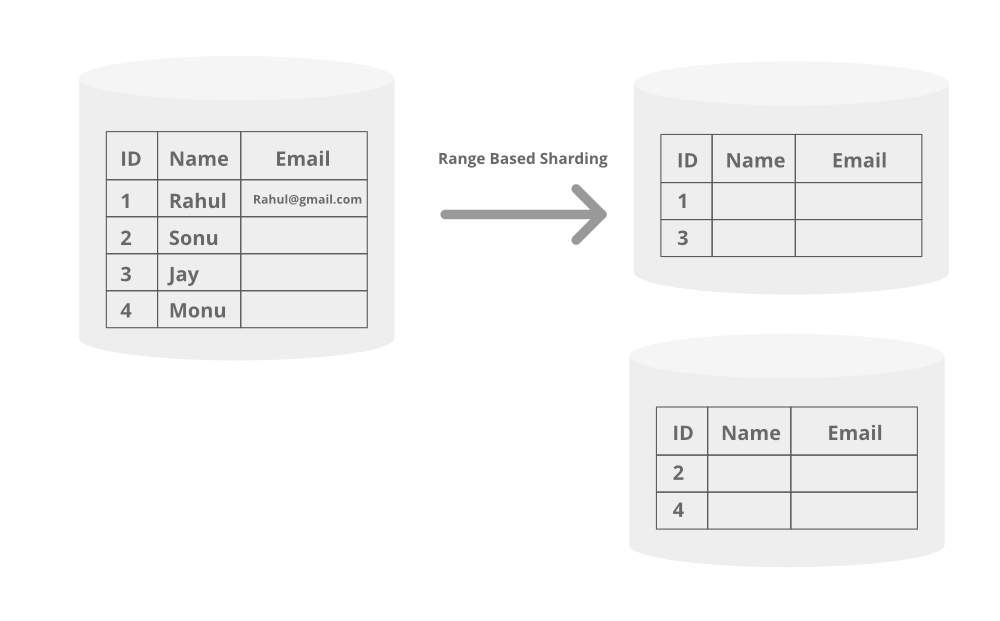
\includegraphics[width=100mm]{assets/distributed/Horizontal-Sharding}
    \caption{Горизонтальное шардирование}
    \label{fig:Horizontal-Sharding}
\end{figure}

\textbf{Горизонтальное шардирование} - самый простой метод сегментирования для реализации. Каждый осколок содержит
другой набор данных, но все они имеют ту же схему, что и исходная база данных. В этом методе вам просто нужно
определить, в какой диапазон попадают ваши данные, а затем вы можете сохранить запись в соответствующий шард. Этот
метод лучше всего подходит для хранения нестатических данных (например, хранение контактной информации студентов
колледжа).

Недостатком этого метода является то, что данные могут быть неравномерно распределены по шардам. В приведенном выше
примере у вас может быть много клиентов, имена которых попадают в категорию A-P. В таких случаях первый осколок должен
будет взять на себя больше нагрузки, чем второй, и это может стать узким местом системы. \autocite{DatabaseSharding}

\paragraph{Вертикальное шардирование} ~\\
В этом методе мы разделяем весь столбец из таблицы и помещаем эти столбцы в новые отдельные таблицы. Данные полностью
независимы от одного раздела к другому. Кроме того, каждый раздел содержит как отдельные строки, так и столбцы. Возьмем,
к примеру, функции Twitter. Мы можем разделить различные функции объекта на разные сегменты на разных машинах. В
Твиттере у пользователя может быть профиль, количество подписчиков и некоторые твиты, опубликованные им самим. Мы можем
разместить профили пользователей на одном осколке, подписчиков - на втором, а твиты - на третьем.

\begin{figure}[H]
    \centering
    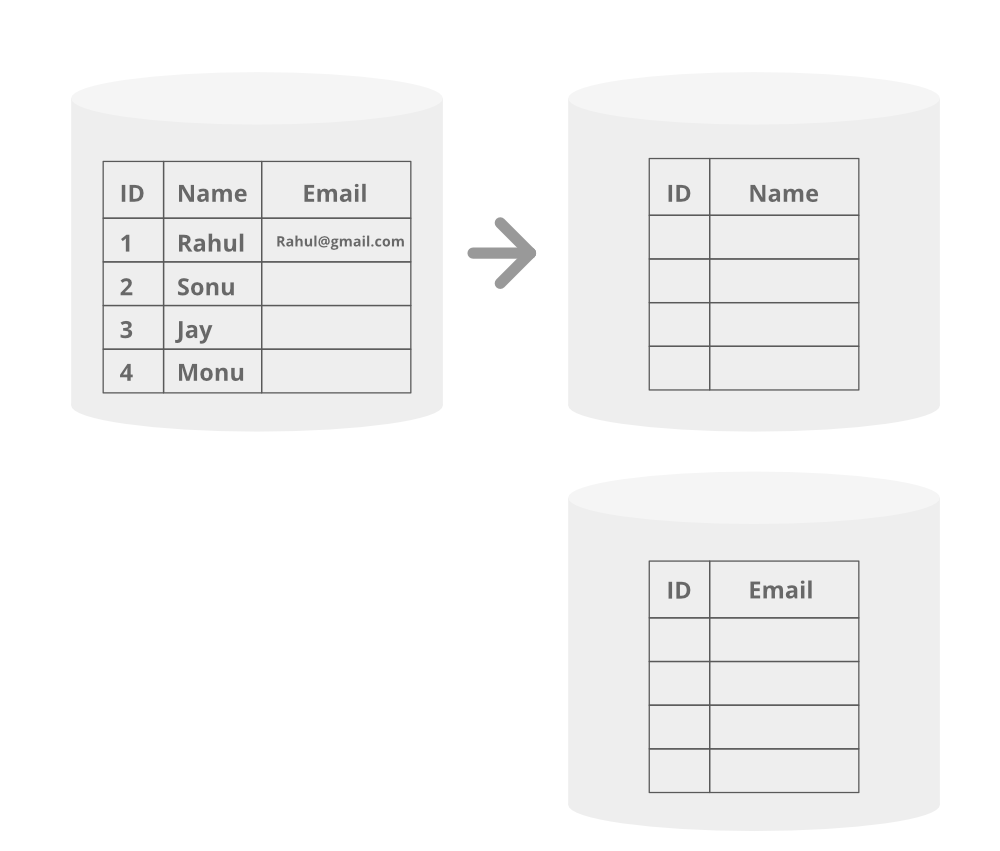
\includegraphics[width=100mm]{assets/distributed/Vertical-Sharding}
    \caption{Вертикальное шардирование}
    \label{fig:Vertical-Sharding}
\end{figure}

В этом методе вы можете отделить и обработать критическую часть (например, профили пользователей) от некритической части
ваших данных (например, сообщения в блоге) по отдельности и построить вокруг нее различные модели репликации и
согласованности. Это одно из главных преимуществ этого метода.

Основным недостатком этой схемы является то, что для ответа на некоторые запросы вам, возможно, придется комбинировать
данные из разных шардов, что неоправданно увеличивает сложность разработки и эксплуатации системы. Кроме того, если
ваше приложение будет расти позже, и вы добавите в него еще несколько функций, вам придется дополнительно сегментировать
базу данных с конкретными функциями на нескольких серверах. \autocite{DatabaseSharding}

\paragraph{Шардинг на основе каталогов} ~\\
В этом методе мы создаем и поддерживаем службу поиска или таблицу поиска для исходной базы данных. В основном мы
используем ключ осколка для таблицы поиска и делаем сопоставление для каждого объекта, существующего в базе данных.
Таким образом, мы отслеживаем, какие осколки базы данных содержат какие данные.

Таблица поиска содержит статический набор информации о том, где можно найти конкретные данные. На приведенном выше
изображении вы можете видеть, что мы использовали зону доставки в качестве ключа осколка. Во-первых, клиентское
приложение запрашивает службу поиска, чтобы узнать осколок (раздел базы данных), на котором размещены данные. Когда
служба поиска возвращает осколок, она запрашивает/обновляет этот осколок.

\begin{figure}[H]
    \centering
    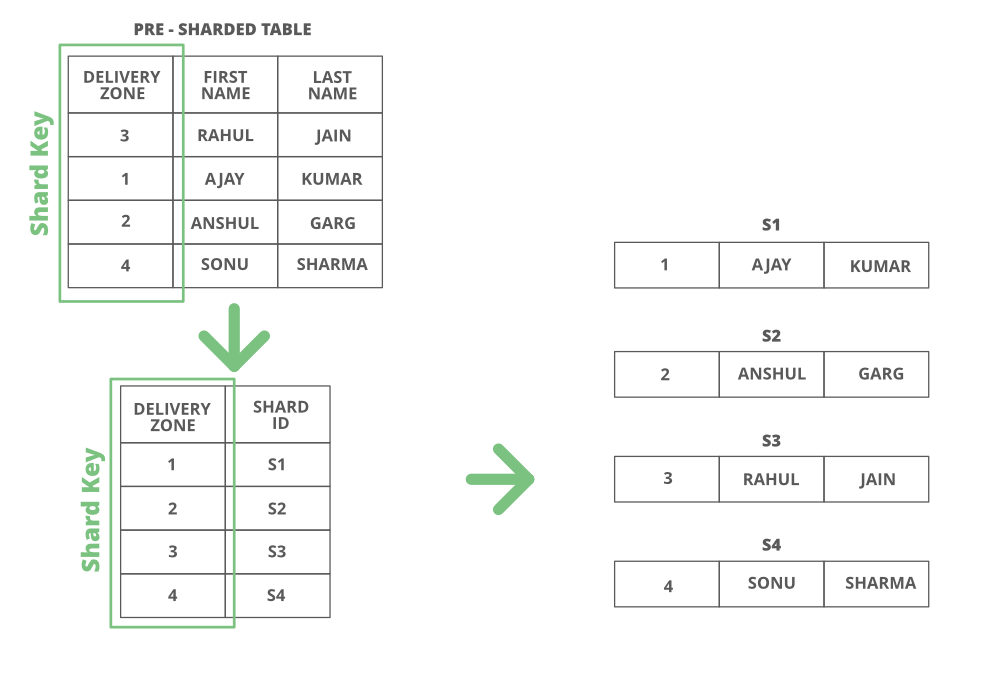
\includegraphics[width=100mm]{assets/distributed/Directory-Based-Sharding}
    \caption{Шардинг на основе каталогов}
    \label{fig:Directory-Based-Sharding}
\end{figure}

Сегментация на основе каталогов гораздо более гибкая, чем сегментация на основе диапазонов и ключей. В сегменте на
основе диапазонов вы обязаны указать диапазоны значений. В key-based вы обязаны использовать фиксированную хэш-функцию,
которую трудно изменить позже. При таком подходе вы можете использовать любой алгоритм, который хотите назначить для
записей данных в сегменты. Кроме того, при таком подходе легко динамически добавлять шарды.

Основным недостатком этого подхода является единственная точка отказа таблицы поиска. Если он будет поврежден или не
удался, это повлияет на запись новых данных или доступ к существующим данным из таблицы. \autocite{DatabaseSharding}

\paragraph{Шардинг на основе ключей} ~\\
Этот метод также известен как сегментация на основе хэша. Здесь мы берем значение объекта, такого как идентификатор
клиента, адрес электронной почты клиента, IP-адрес клиента, почтовый индекс и т. д., и мы используем это значение в
качестве входных данных хэш-функции. Этот процесс генерирует хэш-значение, которое используется для определения того,
какой шард нам нужно использовать для хранения данных. Мы должны иметь в виду, что значения, введенные в хэш-функцию,
должны поступать из одного и того же столбца (ключ осколка), чтобы данные размещались в правильном порядке и
согласованно. В принципе, ключи осколков действуют как первичный ключ или уникальный идентификатор для отдельных строк.

\begin{figure}[H]
    \centering
    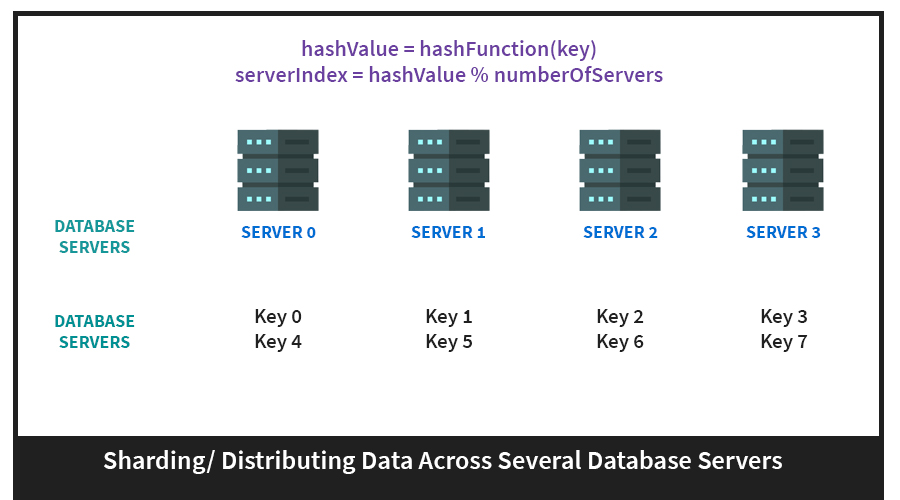
\includegraphics[width=100mm]{assets/distributed/Keybased-Sharding}
    \caption{Шардинг на основе ключей}
    \label{fig:Keybased-Sharding}
\end{figure}

Рассмотрим пример, что у вас есть 3 сервера баз данных, и каждый запрос имеет идентификатор приложения, который
увеличивается на 1 каждый раз, когда регистрируется новое приложение. Чтобы определить, на каком сервере должны быть
размещены данные, мы выполняем операцию по модулю для этих приложений id с номером 3. Затем остаток используется для
идентификации сервера для хранения наших данных.

Недостатком этого метода является эластичная балансировка нагрузки, что означает, если вы попытаетесь динамически
добавлять или удалять серверы баз данных, это будет сложный и дорогостоящий процесс. Например, в приведенном выше
примере, если вы добавите еще 5 серверов, вам нужно добавить больше соответствующих хэш-значений для дополнительных
записей. Кроме того, большинство существующих ключей необходимо переназначить на их новое, правильное хэш-значение,
а затем перенести на новый сервер. Хэш-функция должна быть изменена с модуля 3 на модуль 8. В то время как миграция
данных действует, как новые, так и старые хэш-функции не будут действительны. Во время миграции ваше приложение не
сможет обслуживать большое количество запросов, и вы будете испытывать простои для своего приложения до завершения
миграции. \autocite{DatabaseSharding}

\paragraph{Географический шардинг} ~\\
Шардирование по географическому признаку позволяет хранить определенные данные вблизи своих потребителей и
удовлетворять нормативным требованиям, когда данные должны находиться в определенной юрисдикции. Однако данный способ
шардирования не является самодостаточным: шарды могут быть загружены не равномерно, и отличие может быть на порядки.
На пример, экземпляр базы данных, хранящий данные пользователей Москвы и Московской области, будет намного превышать
другой экземпляр базы данных, который хранит информацию о пользователях из Владимира. Таким образом, недостатком
данного метода является необходимость дополнительного использования других методов шардирования.

\paragraph{Репликация} ~\\
\textbf{Репликация} — это процесс изменения одного набора данных, называемого репликой, в ответ на изменения другого
набора данных, называемого основным. Репликация желательна по крайней мере по двум причинам. Во-первых, она способна
обеспечить более высокую производительность, поскольку приложения смогут обрабатывать локальные копии вместо того,
чтобы устанавливать связь с удаленными узлами. Во-вторых, наличие репликации может также обеспечивать более высокую
степень доступности, поскольку любой реплицируемый объект остается доступным для обработки (по крайней мере, для выборки
данных), пока хотя бы одна реплика в системе остается доступной. Главным недостатком репликации, безусловно, является
то, что если реплицируемый объект обновляется, то и все его копии должны быть обновлены (проблема распространения
обновлений).

Очевидно, что репликация, как и шардирование, теоретически должна быть "прозрачной для пользователя". Другими словами,
система, которая поддерживает репликацию данных, должна также поддерживать независимость от репликации (иногда говорят
"прозрачность репликации"). Для пользователей должна быть создана такая среда, чтобы они, по крайней мере, с логической
точки зрения могли считать, что в действительности данные не дублируются. Независимость от репликации (как и
независимость от шардирования) является весьма желательной, поскольку она упрощает создание пользовательских программ и
выполнение терминальных операций. В частности, независимость от репликации позволяет создавать и уничтожать дубликаты в
любой момент в соответствии с изменяющимися требованиями, не затрагивая при этом никакие из пользовательских программ
или терминальных операций.

Из требования независимости от репликации следует, что к обязанностям системного оптимизатора также относится
определение, какой именно из физических дубликатов будет применен для доступа к данным при выполнении каждого
введенного пользователем запроса. \autocite{IntroBD2014}

Можно выделить три \textbf{подхода к репликации}:
\begin{itemize}
    \item Блочная репликация на уровне системы хранения данных;
    \item Физическая репликация на уровне СУБД;
    \item Логическая репликация на уровне СУБД.
\end{itemize}

\paragraph{Блочная репликация} ~\\
При блочной репликации каждая операция записи выполняется не только на основном диске, но и на резервном. Таким образом
тому на одном массиве соответствует зеркальный том на другом массиве, с точностью до байта повторяющий основной том.

К достоинствам такой репликации можно отнести простоту настройки и надёжность. Записывать данные на удалённый диск может
либо дисковый массив, либо нечто (устройство или программное обеспечение), стоящее между хостом и диском. Если дисковый
массив не способен реплицировать данные, между хостом и массивом может быть установлен агент, осуществляющей запись на
два массива сразу. Агент может быть как отдельным устройством, так и программным компонентом. В отличие от дискового
массива, который может работать только с таким же массивом или, как минимум, с массивом того же производителя, агент
может работать с совершенно разными дисковыми устройствами.

Главное назначение блочной репликации – обеспечение отказоустойчивости. Если база данных потеряна, то можно
перезапустить её с использованием зеркального тома. Блочная репликация хороша своей универсальностью, но за
универсальность приходится платить.

Во-первых, никакой сервер не может работать с зеркальным томом, поскольку его операционная система не может управлять
записью на него; с точки зрения наблюдателя данные на зеркальном томе появляются сами собой. В случае аварии (отказ
основного сервера или всего ЦОДа, где находится основной сервер) следует остановить репликацию, размонтировать основной
том и смонтировать зеркальный том. Как только появится возможность, следует перезапустить репликацию в обратном
направлении.

Во-вторых, сама СУБД на резервном сервере может быть запущена только после монтирования диска. В некоторых операционных
системах, например, в Solaris, память под кеш при выделении размечается, и время разметки пропорционально объёму
выделяемой памяти, то есть старт экземпляра будет отнюдь не мгновенным. Плюс ко всему кеш после рестарта будет пуст.

В-третьих, после запуска на резервном сервере СУБД обнаружит, что данные на диске неконсистентны, и нужно потратить
значительное время на восстановление с применением журналов повторного выполнения: сначала повторить те транзакции,
результаты которых сохранились в журнале, но не успели сохраниться в файлы данных, а потом откатить транзакции, которые
к моменту сбоя не успели завершиться. \autocite{Replication}

\paragraph{Физическая репликация (master-slave)} ~\\
Журналы (redo log или write-ahead log) содержат все изменения, которые вносятся в файлы базы данных. Идея физической
репликации состоит в том, что изменения из журналов повторно выполняются в другой базе (реплике), и таким образом данные
в реплике повторяют данные в основной базе байт-в-байт.

Журналы СУБД не предназначены для использования вне этой платформы, их формат не документируется и может меняться без
предупреждения. Отсюда совершенно естественное требование, что физическая репликация возможна только между экземплярами
одной и той же версии одной той же СУБД. Отсюда же возможные ограничения на операционную систему и архитектуру
процессора, которые тоже могут влиять на формат журнала.

Естественно, никаких ограничений на модели СХД физическая репликация не накладывает. Более того, файлы в базе-реплике
могут располагаться совсем по-другому, чем на базе-источнике – надо лишь описать соответствие между томами, на которых
лежат эти файлы.

Запись данных в реплику невозможна, поскольку изменения в неё приходят побайтно, и реплика не может обеспечить
конкурентное исполнение своих запросов. В случае повреждения файла в основной базе можно просто скопировать
соответствующий файл с реплики. Однако стоит учесть, что файл на реплике может быть не идентичен файлу в основной базе:
когда файл расширяется, новые блоки в целях ускорения ничем не заполняются, и их содержимое случайно. База может
использовать не всё пространство блока (например, в блоке может оставаться свободное место), но содержимое
использованного пространства совпадает с точностью до байта.

Физическая репликация может быть как синхронной, так и асинхронной. При асинхронной репликации всегда есть некий набор
транзакций, которые завершены на основной базе, но ещё не дошли до резервной, и в случае перехода на резервную базу при
сбое основной эти транзакции будут потеряны. При синхронной репликации завершение операции commit означает, что все
журнальные записи, относящиеся к данной транзакции, переданы на реплику. Важно понимать, что получение репликой журнала
не означает применения изменений к данным. При потере основной базы транзакции не будут потеряны, но если приложение
пишет данные в основную базу и считывает их из реплики, то у него есть шанс получить старую версию этих данных.

Физическая репликация базы данных имеет множество преимуществ перед репликацией средствами СХД:
\begin{itemize}
    \item объём передаваемых данных меньше за счёт того, что передаются только журналы, но не файлы с данными; эксперименты показывают уменьшение трафика в 5-7 раз;
    \item переключение на резервную базу происходит значительно быстрее: экземпляр-реплика уже поднят, поэтому при переключении ему нужно лишь откатить активные транзакции; более того, к моменту сбоя кеш реплики уже прогрет;
    \item на реплике можно выполнять запросы, сняв тем самым часть нагрузки с основной базы. В частности, реплику можно использовать для создания резервных копий.
\end{itemize}

\paragraph{Логическая репликация (active-active)} ~\\
Все изменения в базе данных происходят в результате вызовов её API – например, в результате выполнения SQL-запросов.
Очень заманчивой кажется идея выполнять одну и ту же последовательность запросов на двух разных базах. Для репликации
необходимо придерживаться двух правил:
\begin{itemize}
    \item нельзя начинать транзакцию, пока не завершены все транзакции, которые должны закончиться раньше; Так на рисунке ниже нельзя запускать транзакцию D, пока не завершены транзакции A и B;
    \item нельзя завершать транзакцию, пока не начаты все транзакции, которые должны закончиться до завершения текущей транзакции; Так на рисунке ниже даже если транзакция B выполнилась мгновенно, завершить её можно только после того, как начнётся транзакция C.
\end{itemize}

\begin{figure}[H]
    \centering
    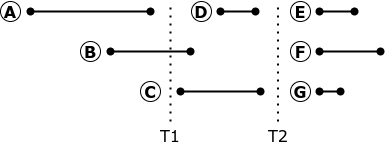
\includegraphics[width=100mm]{assets/distributed/ReplicationExample}
    \caption{Пример репликации}
    \label{fig:ReplicationExample}
\end{figure}

\textbf{Репликация команд (statement-based replication)} реализована, например, в MySQL. К сожалению, эта простая схема не
приводит к появлению идентичных наборов данных – тому есть две причины.
\begin{itemize}
    \item не все API детерминированы. Например, если в SQL-запросе встречается функция now() или sysdate(), возвращающая текущее время, то на разных серверах она вернёт разный результат – из-за того, что запросы выполняются не одновременно. Кроме того, к различиям могут привести разные состояния триггеров и хранимых функций, разные национальные настройки, влияющие на порядок сортировки, и многое другое.
    \item репликацию, основанную на параллельном исполнении команд, невозможно корректно приостановить и перезапустить. На рисунке выше если репликация остановлена в момент T1 транзакция B должна быть прервана и откачена. При перезапуске репликации исполнение транзакции B может привести реплику к состоянию, отличному от состояния базы-источника: на источнике транзакция B началась до того, как закончилась транзакция A, а значит, она не видела изменений, сделанных транзакцией A. Репликация запросов может быть остановлена и перезапущена только в момент T2, когда в базе нет ни одной активной транзакции. Разумеется, на сколько-нибудь нагруженной промышленной базе таких моментов не бывает.
\end{itemize}

Обычно для логической репликации используют детерминированные запросы. Детерминированность запроса обеспечивается двумя
свойствами:
\begin{itemize}
    \item запрос обновляет (или вставляет, или удаляет) единственную запись, идентифицируя её по первичному (или уникальному) ключу;
    \item все параметры запроса явно заданы в самом запросе.
\end{itemize}

В отличие от \textbf{репликации команд (statement-based replication)} такой подход называется \textbf{репликацией
записей (row-based replication)}.

База-реплика открыта и доступна не только на чтение, но и на запись. Это позволяет использовать реплику для выполнения
части запросов, в том числе для построения отчётов, требующих создания дополнительных таблиц или индексов. Важно
понимать, что логическая реплика будет эквивалентна исходной базе только в том случае, если в неё не вносится никаких
дополнительных изменений

Логическая репликация предоставляет ряд возможностей, отсутствующих в других видах репликации:
\begin{itemize}
    \item настройка набора реплицируемых данных на уровне таблиц (при физической репликации – на уровне файлов и табличных пространств, при блочной репликации – на уровне томов);
    \item построение сложных топологий репликации – например, консолидация нескольких баз в одной или двунаправленная репликация;
    \item уменьшение объёма передаваемых данных;
    \item репликация между разными версиями СУБД или даже между СУБД разных производителей;
    \item обработка данных при репликации, в том числе изменение структуры, обогащение, сохранение истории.
\end{itemize}

Есть и недостатки, которые не позволяют логической репликации вытеснить физическую:
\begin{itemize}
    \item все реплицируемые данные обязаны иметь первичные ключи;
    \item логическая репликация поддерживает не все типы данных;
    \item логическая репликация на практике не бывает полностью синхронной: время от получения изменений до их применения слишком велико, чтобы основная база могла ждать;
    \item логическая репликация создаёт большую нагрузку на реплику;
    \item при переключении приложение должно иметь возможность убедиться, что все изменения с основной базы, применены на реплике – СУБД зачастую сама не может этого определить, так как для неё режимы реплики и основной базы эквивалентны.
\end{itemize}

Два последних недостатка существенно ограничивают использование логической реплики как средства отказоустойчивости. Если
один запрос в основной базе изменяет сразу много строк, реплика может существенно отставать. А возможность смены ролей
требует недюжинных усилий как со стороны разработчиков, так и со стороны администраторов.

Есть несколько способов реализации логической репликации, и каждый из этих способов реализует одну часть возможностей и
не реализует другую:
\begin{itemize}
    \item репликация триггерами;
    \item использование журналов СУБД;
    \item использование программного обеспечения класса CDC (change data capture);
    \item прикладная репликация.
\end{itemize}

\paragraph{Репликация триггерами} ~\\
Триггер – хранимая процедура, которая исполняется автоматически при каком-либо действии по модификации данных. Триггеру,
который вызывается при изменении каждой записи, доступны ключ этой записи, а также старые и новые значения полей. При
необходимости триггер может сохранять новые значения строк в специальную таблицу, откуда специальный процесс на стороне
реплики будет их вычитывать

\textbf{Преимущества}:
\begin{itemize}
    \item независимость от версий основной базы и реплики;
    \item широкие возможности преобразования данных.
\end{itemize}

\textbf{Недостатки}:
\begin{itemize}
    \item нагрузка на основную базу;
    \item большая задержка при репликации.
\end{itemize}

\paragraph{Использование журналов СУБД} ~\\
Сами СУБД также могут предоставлять возможности логической репликации. Источником данных, как и для физической
репликации, являются журналы. К информации о побайтовом изменении добавляется также информация об изменённых полях, а
также значение уникального ключа, даже если он не меняется. В результате объём журналов БД увеличивается – по разным
оценкам от 10 до 15%.

К \textbf{недостаткам} данного подхода можно отнести увеличение объёма журналов и возможное увеличение трафика между
узлами.

\paragraph{Использование CDC} ~\\
Существует целый класс программного обеспечения, предназначенного для организации логической репликации. Это ПО
называется CDC, change data capture. В задачу платформы входит чтение журналов базы данных, преобразование информации,
передача информации на реплику и применение. Как и в случае репликации средствами самой СУБД, журнал должен содержать
информацию об изменённых полях. Использование дополнительного приложения позволяет «на лету» выполнять сложные
преобразования реплицируемых данных и строить достаточно сложные топологии репликации.

\textbf{Преимущества}:
\begin{itemize}
    \item возможность репликации между разными СУБД, в том числе загрузка данных в отчётные системы;
    \item широчайшие возможности обработки и преобразования данных;
    \item минимальный трафик между узлами – платформа отсекает ненужные данные и может сжимать трафик;
    \item встроенные возможности мониторинга состояния репликации.
\end{itemize}

\textbf{Недостатки}:
\begin{itemize}
    \item увеличение объёма журналов, как при логической репликации средствами СУБД;
    \item новое ПО – сложное в настройке и/или с дорогими лицензиями.
\end{itemize}

\paragraph{Прикладная репликация} ~\\
Наконец, ещё один способ репликации – формирование векторов изменений непосредственно на стороне клиента. Клиент должен
формировать детерминированные запросы, затрагивающие единственную запись. Добиться этого можно, используя специальную
библиотеку работы с базой данных. Когда приложение завершает транзакцию, специально подключаемый модуль записывает
вектор изменений в очередь и выполняет транзакцию в базе данных. Специальный процесс-репликатор вычитывает векторы из
очереди и выполняет транзакции в базе-реплике.Этот механизм хорош для обновления отчётных систем. Может он
использоваться и для обеспечения отказоустойчивости, но в этом случае в приложении должен быть реализован контроль
состояния репликации

\textbf{Преимущества}:
\begin{itemize}
    \item возможность репликации между разными СУБД, в том числе загрузка данных в отчётные системы;
    \item возможность обработки и преобразования данных, мониторинга состояния и т. д.;
    \item минимальный трафик между узлами – платформа отсекает ненужные данные и может сжимать трафик;
    \item полная независимость от базы данных – как от формата, так и от внутренних механизмов.
\end{itemize}

\textbf{Недостатки}:
\begin{itemize}
    \item ограничения на архитектуру приложения;
    \item огромный объём собственного кода, обеспечивающего репликацию.
\end{itemize}

\paragraph{Сравнение подходов к репликации} ~\\
Описав все подходы к репликации, можно установить следующее:
\begin{itemize}
    \item \textbf{Блочная репликация} имеет смысл, когда других способов репликации нет; для баз данных её лучше не использовать.
    \item \textbf{Физическая репликация} хороша, когда требуется обеспечение отказоустойчивости инфраструктуры или перенос части читающих приложений на реплики.
    \item \textbf{Логическая репликация} подходит для обеспечения отказоустойчивости только в том случае, если приложение знает об этой репликации и умеет в случае аварии ждать синхронизации реплик.
    \item \textbf{Логическая репликация} идеальна для всевозможных отчётных баз.
    \item \textbf{Репликация триггерами} имеет смысл в том случае, если база сильно нагружена, а реплицировать нужно крайне ограниченное количество информации.
    \item \textbf{Платформы CDC} хороши, если у вас большое количество реплицируемых баз и/или есть необходимость сложных преобразований данных.
    \item Разработка \textbf{прикладной репликации} оправдана только в случае разработки собственной платформы или фреймворка.
\end{itemize} \autocite{Replication}

\paragraph{Greenplum} ~\\
Ранее уже сравнивались различные подходы шардирования между собой. Сравнивались различные подходы репликации между
собой. Осталось только сравнить способы тиражирования, то есть сравнить репликацию и шардирование.

Вообще говоря, шардинг и репликация не противоречат друг другу и могут сосуществовать. Они выполняют разные задачи, и
сравнивать их не имеет смысла. Репликация используется для ускорения взаимодействия с бд с помощью использования копий
основной базы данных. Кроме того, репликация осуществляет отказоустойчивость. В свою очередь шардинг осуществляет
ускорение работы с базой данных с помощью разбиения исходной базы данных на несколько разных, хранящихся на разных
серверах.  Шардирование не реализует отказоустойчивость.

В принципе, на этом их сравнение можно закончить и перейти к примеру. Один из классических примеров в котором
реализовано сочетание репликации и шардирования - \textbf{Greenplum}.

\textbf{Greenplum (GP)} – реляционная СУБД, имеющая массово-параллельную (massive parallel processing) архитектуру без
разделения ресурсов (Shared Nothing). В общем случае кластер GP состоит из нескольких серверов-сегментов (именно
сегменты непосредственно хранят данные, выполняют с ними операции и отдают результаты мастеру (в общем случае). По сути
сегмент – самый обычный инстанс PostgreSQL 8.2.15 с настроенной логической репликацией в своё зеркало на другом
сервере), одного сервера-мастера (сервер, на котором работает инстанс, являющийся одновременно координатором и входной
точкой для пользователей в кластере), и одного сервера-секондари-мастера (инстанс, являющийся резервным мастером,
включается в работу в случае недоступности основного мастера (переключение происходит вручную)), соединённых между
собой одной или несколькими быстрыми (10g, infiniband) сетями, обычно обособленными (interconnect). На рисунке ниже
представлен состав кластера и сетевое взаимодействие элементов. Здесь — зелёная и красная линии — обособленные сети
interconnect, синяя линия — внешняя, клиентская сеть.

\begin{figure}[H]
    \centering
    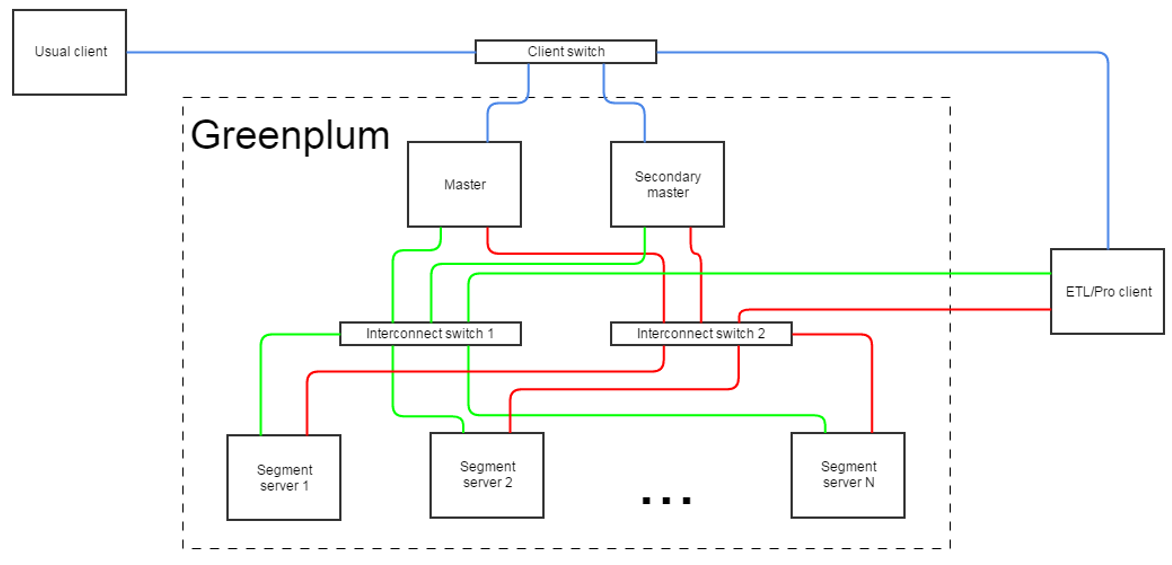
\includegraphics[width=100mm]{assets/distributed/Greenplum}
    \caption{Состав кластера и сетевое взаимодействие элементов Greenplum}
    \label{fig:Greenplum}
\end{figure}

При выборе числа серверов-сегментов важно правильно выбрать соотношение кластера «число процессоров/Тб данных» в
зависимости от планируемого профиля нагрузки на БД — чем больше процессорных ядер приходится на единицу данных, тем
быстрее кластер будет выполнять «тяжёлые» операции, а также работать со сжатыми таблицами.

При выборе числа сегментов в кластере (которое в общем случае к числу серверов никак не привязано) необходимо помнить
следующее:
\begin{itemize}
    \item все ресурсы сервера делятся между всеми сегментами на сервере (нагрузкой зеркал, в случае если они располагаются на этих же серверах, можно условно пренебречь);
    \item каждый запрос на одном сегменте не может потреблять процессорных ресурсов больше, чем одно ядро CPU. Это означает, например, что, если кластер состоит из 32-ядерных серверов с 4-я сегментами GP на борту и используется в среднем для обработки 3-4 одновременных тяжёлых, хорошо утилизирующих CPU, запросов, «в среднем по больнице» CPU не будет утилизироваться оптимально. В данной ситуации лучше увеличить число сегментов на сервере до 6-8;
    \item штатный процесс бекапа и рестора данных «из коробки» работает только на кластерах, имеющих одинаковое число сегментов. Восстановить данные, забекапленные на кластере из 96 сегментов, в кластер из 100 сегментов без напильника будет невозможно.
\end{itemize}

В Greenplum реализуется классическая схема шардирования данных. Каждая таблица представляет из себя N+1 таблиц на всех
сегментах кластера, где N – число сегментов (+1 в этом случае — это таблица на мастере, данных в ней нет). На каждом
сегменте хранится 1/N строк таблицы. Логика разбиения таблицы на сегменты задаётся ключом (полем) дистрибуции – таким
полем, на основе данных которого любую строку можно отнести к одному из сегментов.

По подробнее почитать про Greenplum можно в источнике. В данной главе приведена только краткая информация об общей
архитектуре и информация, относящаяся к тиражированию данных. \autocite{Greenplum}

\subsection{Интеграция БД и Internet}
\paragraph{Современные тенденции}
\paragraph{Обзор существующих технологий}
\paragraph{Вопросы безопасности: угрозы и методы противодействия}
\paragraph{Перспективы развития}